%% document
\documentclass[11pt]{article}
\usepackage[letterpaper, portrait, margin=0.75in]{geometry}
\usepackage{setspace}
\usepackage{color}

% text
\usepackage[utf8]{inputenc}
\setlength\parindent{0pt}
\setlength{\parskip}{1em}
\renewcommand{\familydefault}{\sfdefault}
\newcommand{\RomanNumeral}[1]{\textrm{\uppercase\expandafter{\romannumeral #1\relax}}}

% math
\usepackage{amssymb}
\usepackage{amsmath}
\usepackage[cm]{sfmath}
\usepackage{commath}
\usepackage{multirow}
\DeclareMathAlphabet{\mathpzc}{OT1}{pzc}{m}{it}

% graphics
\usepackage{graphics}
\usepackage{graphicx}
\usepackage{epsfig}
\usepackage{epstopdf}
\usepackage{xpatch}
\usepackage{pdfpages}
\usepackage{float}

% each section begins new page
\let\stdsection\section
\renewcommand\section{\clearpage\stdsection}

% hyperref
\usepackage[colorlinks=true, linkcolor=black, urlcolor=blue, citecolor=black, anchorcolor=black]{hyperref}
\usepackage[all]{hypcap}  % helps hyperref work properly



\usepackage[shortlabels]{enumitem}
\setlist[enumerate, 1]{nosep}
\setlist[enumerate, 2]{nosep, topsep=-5ex}
\setlist[enumerate, 3]{nosep, topsep=-5ex}
\setlist[enumerate, 4]{nosep, topsep=-5ex}
\setlist[itemize, 1]{nosep}
\setlist[itemize, 2]{nosep, topsep=-5ex}
\setlist[itemize, 3]{nosep, topsep=-5ex}
\setlist[itemize, 4]{nosep, topsep=-5ex}

% bibliography
\usepackage[numbers]{natbib}

% title
\title{Wisconsin Photoreactor Platform\\Fabrication and Operation Guide}
\author{
  Philip P. Lampkin \\
  Blaise J. Thompson \\
  Samuel H. Gellman
  }
\date{\today}

\begin{document}

\maketitle


\includegraphics[width=\textwidth]{"../coverart.png"}

\tableofcontents

\section{Introduction}

Below are instructions for fabrication, operation and documentation of Wisconsin Photoreactor Platform (WPP) devices. 

For access to all project source files, documentation and resources, visit the Wisconsin Photoreactor Platform project repository on GitHub at \href{https://github.com/uw-madison-chem-shops/wisconsin-photoreactor}{https://github.com/uw-madison-chem-shops/wisconsin-photoreactor}. 

\begin{figure}[H]
	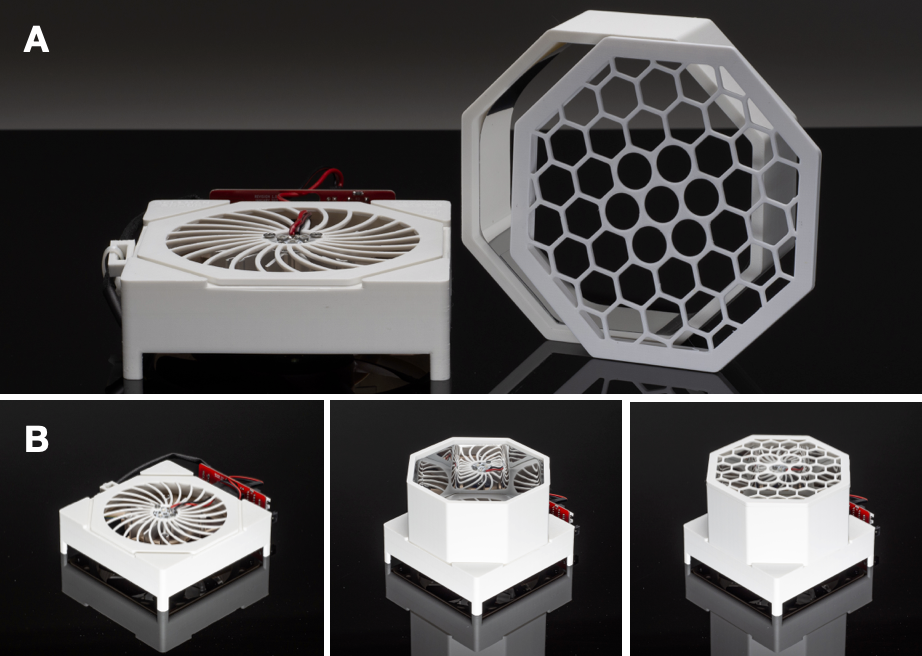
\includegraphics[width=\textwidth]{"./fig1.png"}
	\caption{(A) Unassembled WPP device comprised of a vessel holder, reaction chamber and standardized base fitted with a digital driver board. (B) Modular apparatus assembly.}
\end{figure}
A WPP device consists of a base, reaction module and reactor driver (Figure 1A).
The base houses the photon source and cooling fan.
The reaction module is comprised of a reflective reaction chamber and rigid vessel holder.
A digital driver board, analog driver board or simple circuit integrating a commercial light emitting diode (LED) driver can be fitted to the base to drive the reactor.

Each component is highly versatile, and apparatus assembly is fully modular (Figure 1B).
Through variation of each component, one can quickly produce bespoke WPP devices to meet specific research needs.

The WPP is a living project.
We encourage duplication and modification of our designs.
If you would like to contribute to the WPP project or notice an issue, please consider opening an pull request or issue on GitHub.

\section{Fabrication}

WPP devices are simple to fabricate.
To fabricate a WPP device, you'll need a soldering iron, electronics tweezers, thin nose pliers and a screwdriver. 
The fabrication process is divided into three parts:

\begin{itemize}
	\item Base fabrication, described in \autoref{SEC:base}
	\item Reaction module fabrication, described in \autoref{SEC:enclosure}
	\item Reactor driver electronics fabrication, described in \autoref{SEC:electronics}
\end{itemize}

With these components complete, final assembly of WPP devices is straightforward.
Details of the final assembly process are described in \autoref{SEC:assembly}.

A WPP device is made up of many separate commercially available parts.
This guide assumes that you have already procured those parts.
The project repository provides README files containing a bill of materials for each component with detailed part numbers and suggested vendors.

\subsection{Base Fabrication} \label{SEC:base}

\begin{figure}[H]
	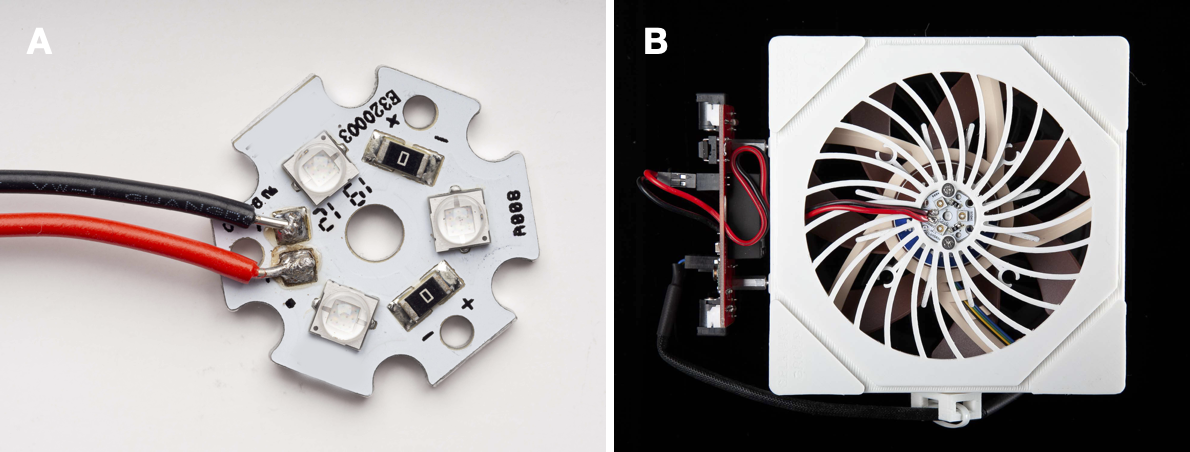
\includegraphics[width=\textwidth]{"./fig2.png"}
	\caption{(A) Commercial 20 mm LED star mounted with 450 nm Cree, Inc. XT-E LEDs. (B) Top-down view of WPP base depicting integrated LED star.}
\end{figure}

The WPP architecture uses industry standard 20 mm ``LED star'' circuit boards mounted with 3 high-intensity LEDs to deliver photons to photoreactions (Figure 2A).
LED stars are commercially available or can be easily fabricated. 
The range of wavelengths provided by a LED star depends upon the emission profile of the mounted LEDs.
\textbf{\textit{Through variation of the LED star integrated into a WPP base (Figure 2B), the user can control the wavelengths of light delivered by the photon source to a reaction vessel.}}
An aluminim heatsink and cooling fan are integrated to keep the LED star from overheating. 

A list of LED stars tested with the WPP platform is available in the 'photon-source-leds' subdirectory of the project repository. 
It is easiest to use LED stars with pre-mounted LEDs.
Otherwise, you can order discrete LEDs and bare LED star circuit boards to fabricate your own.
Custom LED star production requires a reflow oven. 
All LED stars must be mounted with LEDs with a maximum forward current of 1000 mA.

\begin{figure}[H]
	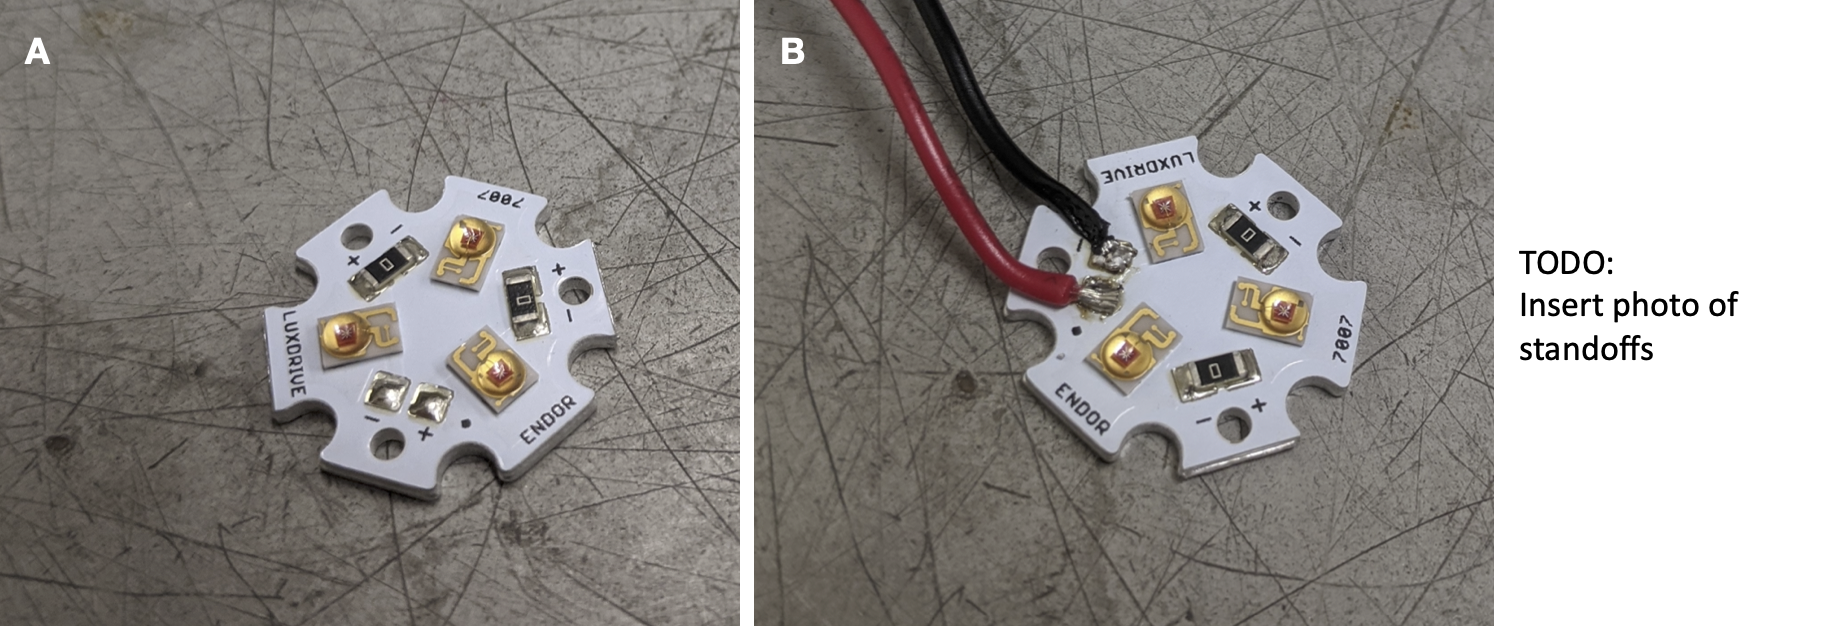
\includegraphics[width=\textwidth]{"./fig3.png"}
	\caption{(A) Unsoldered commerical LED star. (B) LED star with leads. (C) Connectors on other end of leads. (D) Connector sealed with heat-shrink tubing.}
\end{figure}

Fabrication of a WPP base begins with preparation of an LED star.
Solder leads onto your LED star, using the red positive and black negative convention (Figure 3A---B).
We recommend 22 gauge solid core wire.
This is often sold as "standard hookup wire"
Soldering may be challenging, as the LED star itself will resist efforts to heat it.
Using lead-based solder with a low melting point may help.

Solder a connector to the end of the LED star. 
Ensure the connection between the connector and wire is strong and has plenty of sodler ()Figure 3C).
Using heat-shrink tubing, seal the connector and wire junction (Figure 3D).

\begin{figure}[H]
	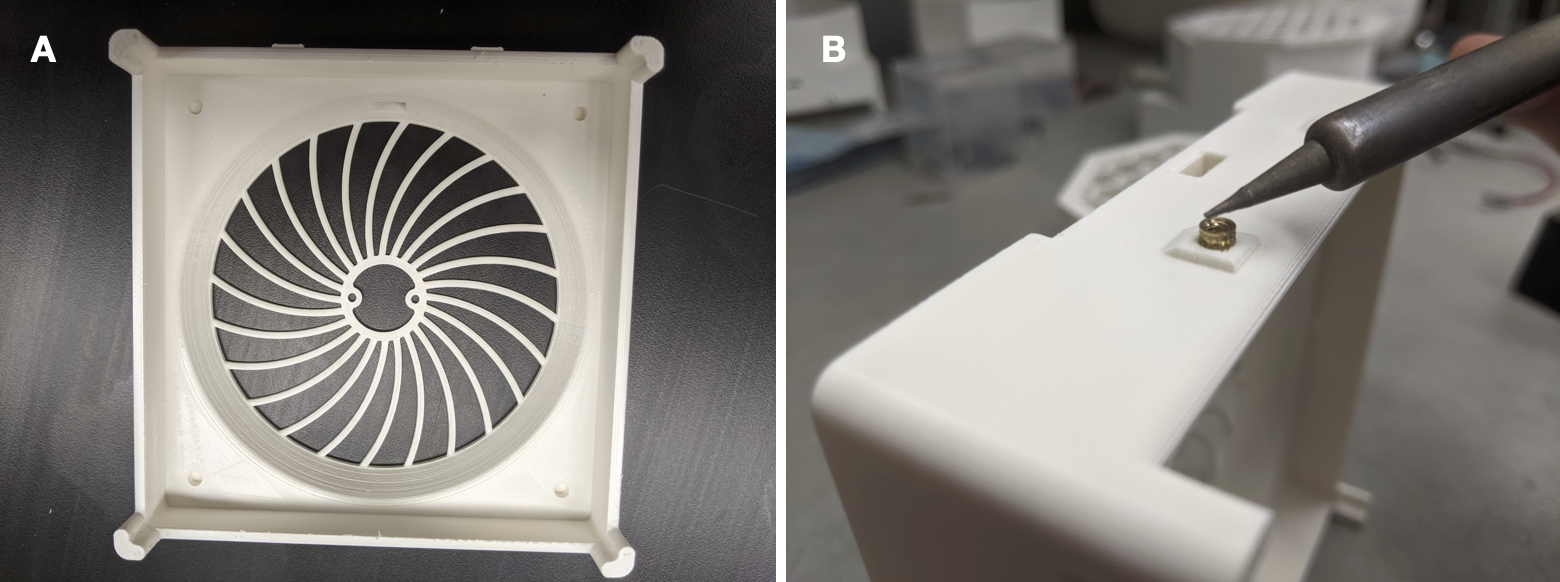
\includegraphics[width=\textwidth]{"./fig4.png"}
	\caption{(A) 3D-printed WPP base. (B) Securing a threaded inset into base.}
\end{figure}

Next, 3D-print the enclosure base and cable anchor models provided in the 'photoreactor-base' subdirectory of the project repository (Figure 4A).
The same base is shared by all WPP devices.

When interacting with the design files in our repository you will see several filetypes.
We have designed the WPP enclosure using Fusion 360, and included f3d design source files for those that wish to extend or modify our designs.
Interacting with f3d files requires use of Fusion 360 license.
You will also find stl files in the repository.
These are common 3D-model exchange files which can be viewed with 3D modeling programs or printed with 3D-printers. 

We recommend white PLA as the printing material. We have also used white ABS.
If you are printing yourself, follow the instructions provided by your 3D-printer's manufacturer.
You will need to enable support material for printing the base.
Any company or shop offering 3D printing as a service should accept our stl files without modification.
Once your base is printed you may need to remove excess material with a razor blade or exacto-knife.

We have succesfully printed using the following printers:

\begin{itemize}
	\item Creality Ender 3
	\item Stratasys uPrint SE Plus
	\item Ultimaker 3 Extended
\end{itemize}

Each base contains seven threaded heat inserts.
These allow components such as the drive circuit board to rigidly attach to the base via machine screws.
Use a soldering iron to carefully heat these while pushing them into their cavities (Figure 4B).

\begin{figure}[H]
	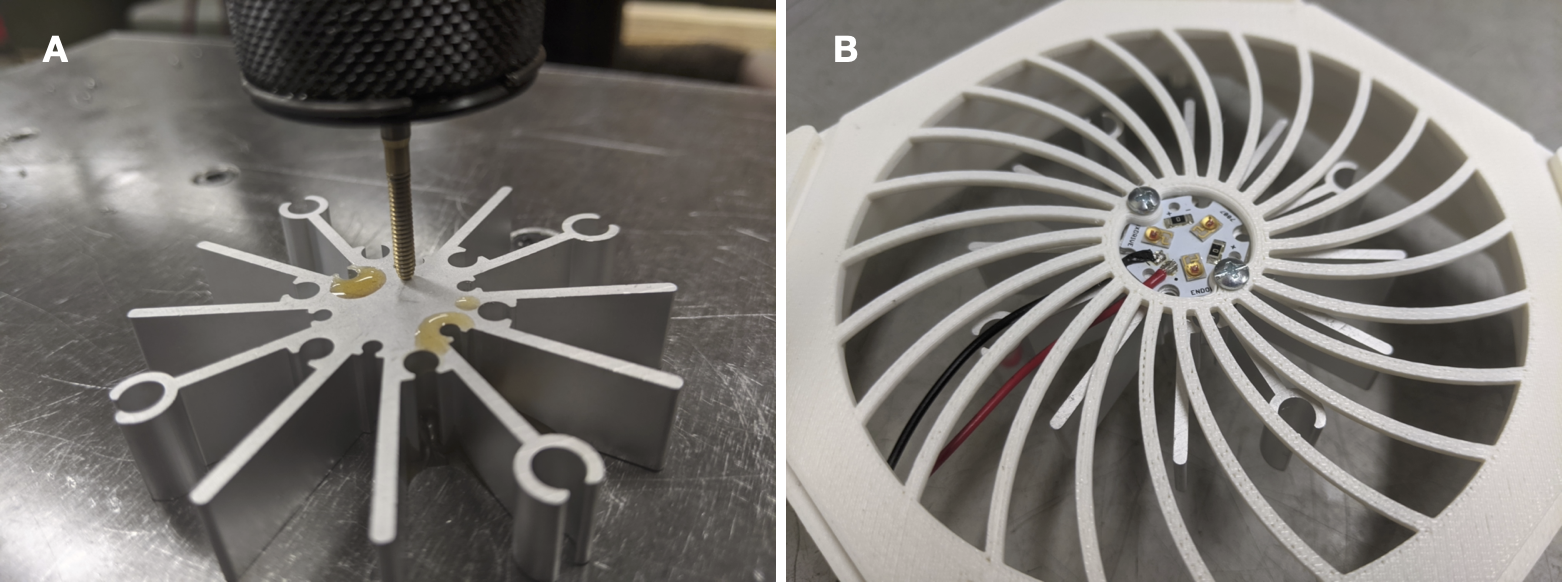
\includegraphics[width=\textwidth]{"./fig5.png"}
	\caption{(A) Tapping aluminium heatsink. (B) LED star and heatsink installed into WPP base.}
\end{figure}

Now tap an aluminum heatsink for imperial 4-40 machine screws.
We used thread-forming tap: OSG 1400105300 with a pneumatic ``air-tapper'' (Figure 4).
The heatsink can be tapped by hand.
You only need to tap two of the innermost holes.

Install the LED star and heatsink into the WPP base using 1/4'' screws.
Ensure the LED wires face towards the hole in the side of the printed base.  

\begin{figure}[H]
	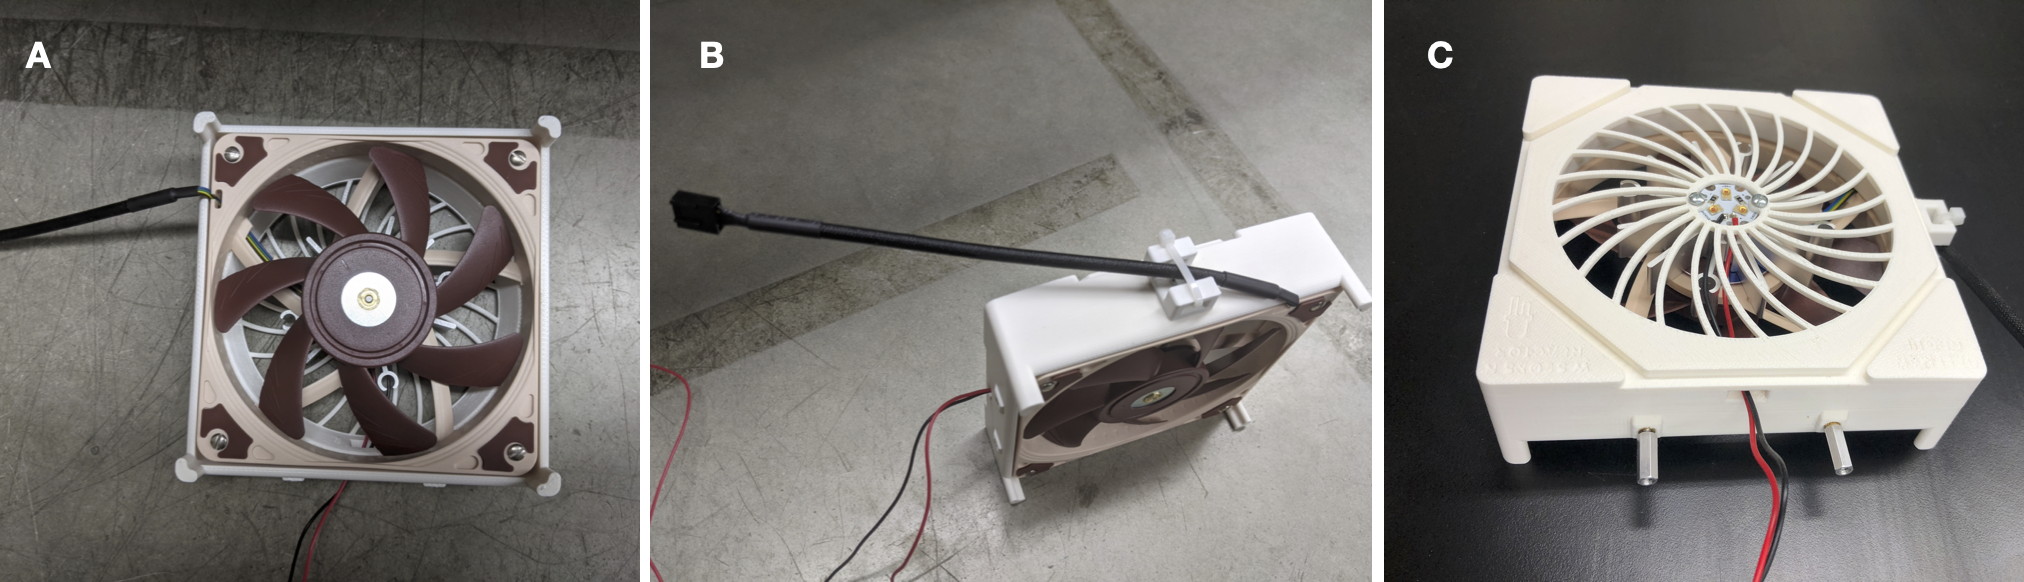
\includegraphics[width=\textwidth]{"./fig6.png"}
	\caption{(A) Integrated Fan. (B) Installed cable anchor with captured fan cord. (C) Metal standoffs screwed into base.}
\end{figure}

Install the fan.
Pay special attention to the orientation of the fan, including the location of the cord (Figure 6A).
Use 3/4'' screws here.
Then, install the cable anchor using a 1/4'' screw.
Use a zip tie to capture the fan cord (Figure 6B).
Finally, screw in the threaded standoffs (Figure 6C). 
Your WPP base is now ready for use.

\begin{figure}[H]
	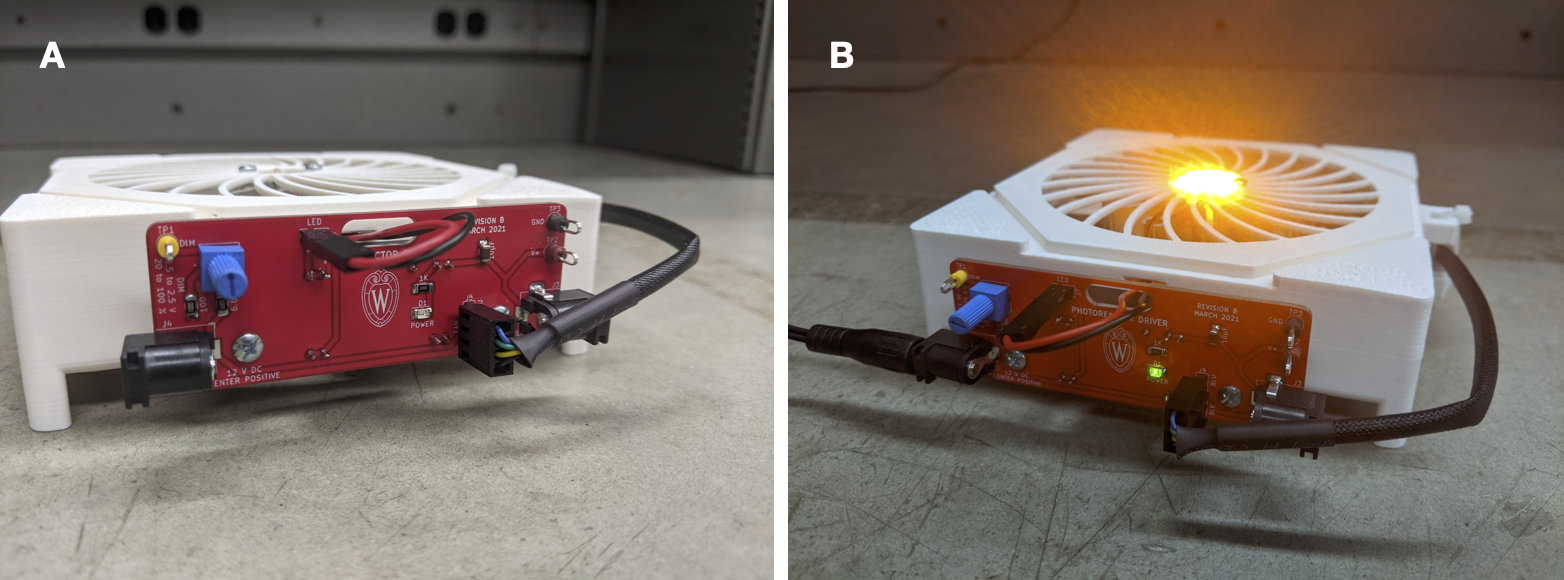
\includegraphics[width=\textwidth]{"./fig7.png"}
	\caption{A WPP base fitted with an analog driver board with and without power.}
\end{figure}

To test the photoreactor base, simply screw a driver board to the threaded standoffs and plug the LED and fan into the board.
Pay special attention to the orientation of both connectors.
Your base should light up upon connection to power (Figure 7).
Remember to use proper eye protection.

\clearpage

\subsection{Reaction Module} \label{SEC:enclosure}

\begin{figure}[H]
	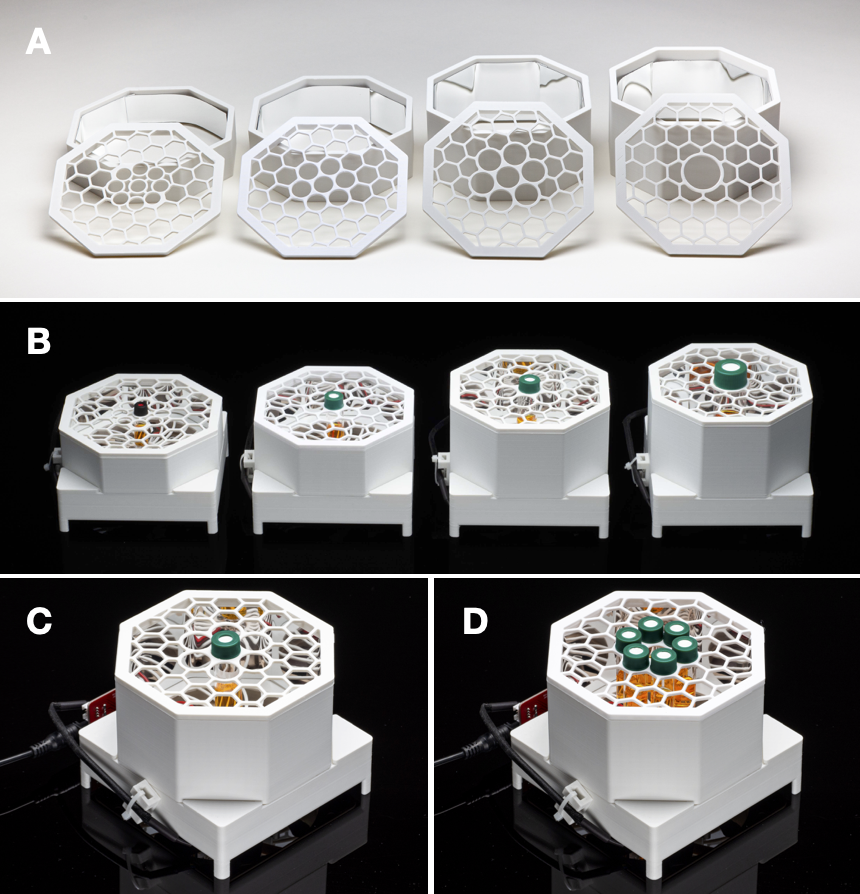
\includegraphics[width=\textwidth]{"./fig8.png"}
	\caption{(A) Provided reaction modules for 1-, 4-, 8- and 24-mL vials. (B) WPP devices fitted with the provided reaction modules. (C) Single and (D) multiple reaction configurations for provide 4-mL module.}
\end{figure}

A WPP reaction module consists of a reaction chamber and vessel holder.
By modifying chamber height and adjusting holder geometry, one can produce modules compatible with reaction vessels of various types and sizes.
Template reaction chamber and vessel holder Fusion360 designs are provided in the project repository.
Fusion360 designs and stl models for modules compatible with 1-, 4-, 8- and 24-mL vials are provided in the 'photoreaction-modules' subdirectory of the project repository (Figure 8A—B).

We encourage you to design your own if none of these suit your application.
Consider adding your new designs to WPP repository so that others may benefit from your design efforts.

A single reaction module can offer multiple layouts for reaction vessel placement.
For the provided modules, two vessel placement configurations exist.
First, the single reaction configuration, where one vessel is placed in the center of the module directly above the photon source (Figure 8C).
This configuration exposes one vessel to maximum light intensity.
Second, the multiple reaction configuration, where multiple vessels are placed in a circle around the photon source (Figure 8D).
This configuration exposes each vessel to less light relative to the single reaction configuration but provides equivalent exposure to each vessel.
\textbf{\textit{Through variation of the reaction module, the user can configure the reaction vessel type, size and placement within a WPP apparatus.}}

To fabricate a reaction module, simply 3D-print a reaction chamber and vial holder models. You can use those supplied in the 'photoreaction-modules' subdirectory or design your own using the templates designs in the same subdirectory. 

\begin{figure}[H]
	\centering
	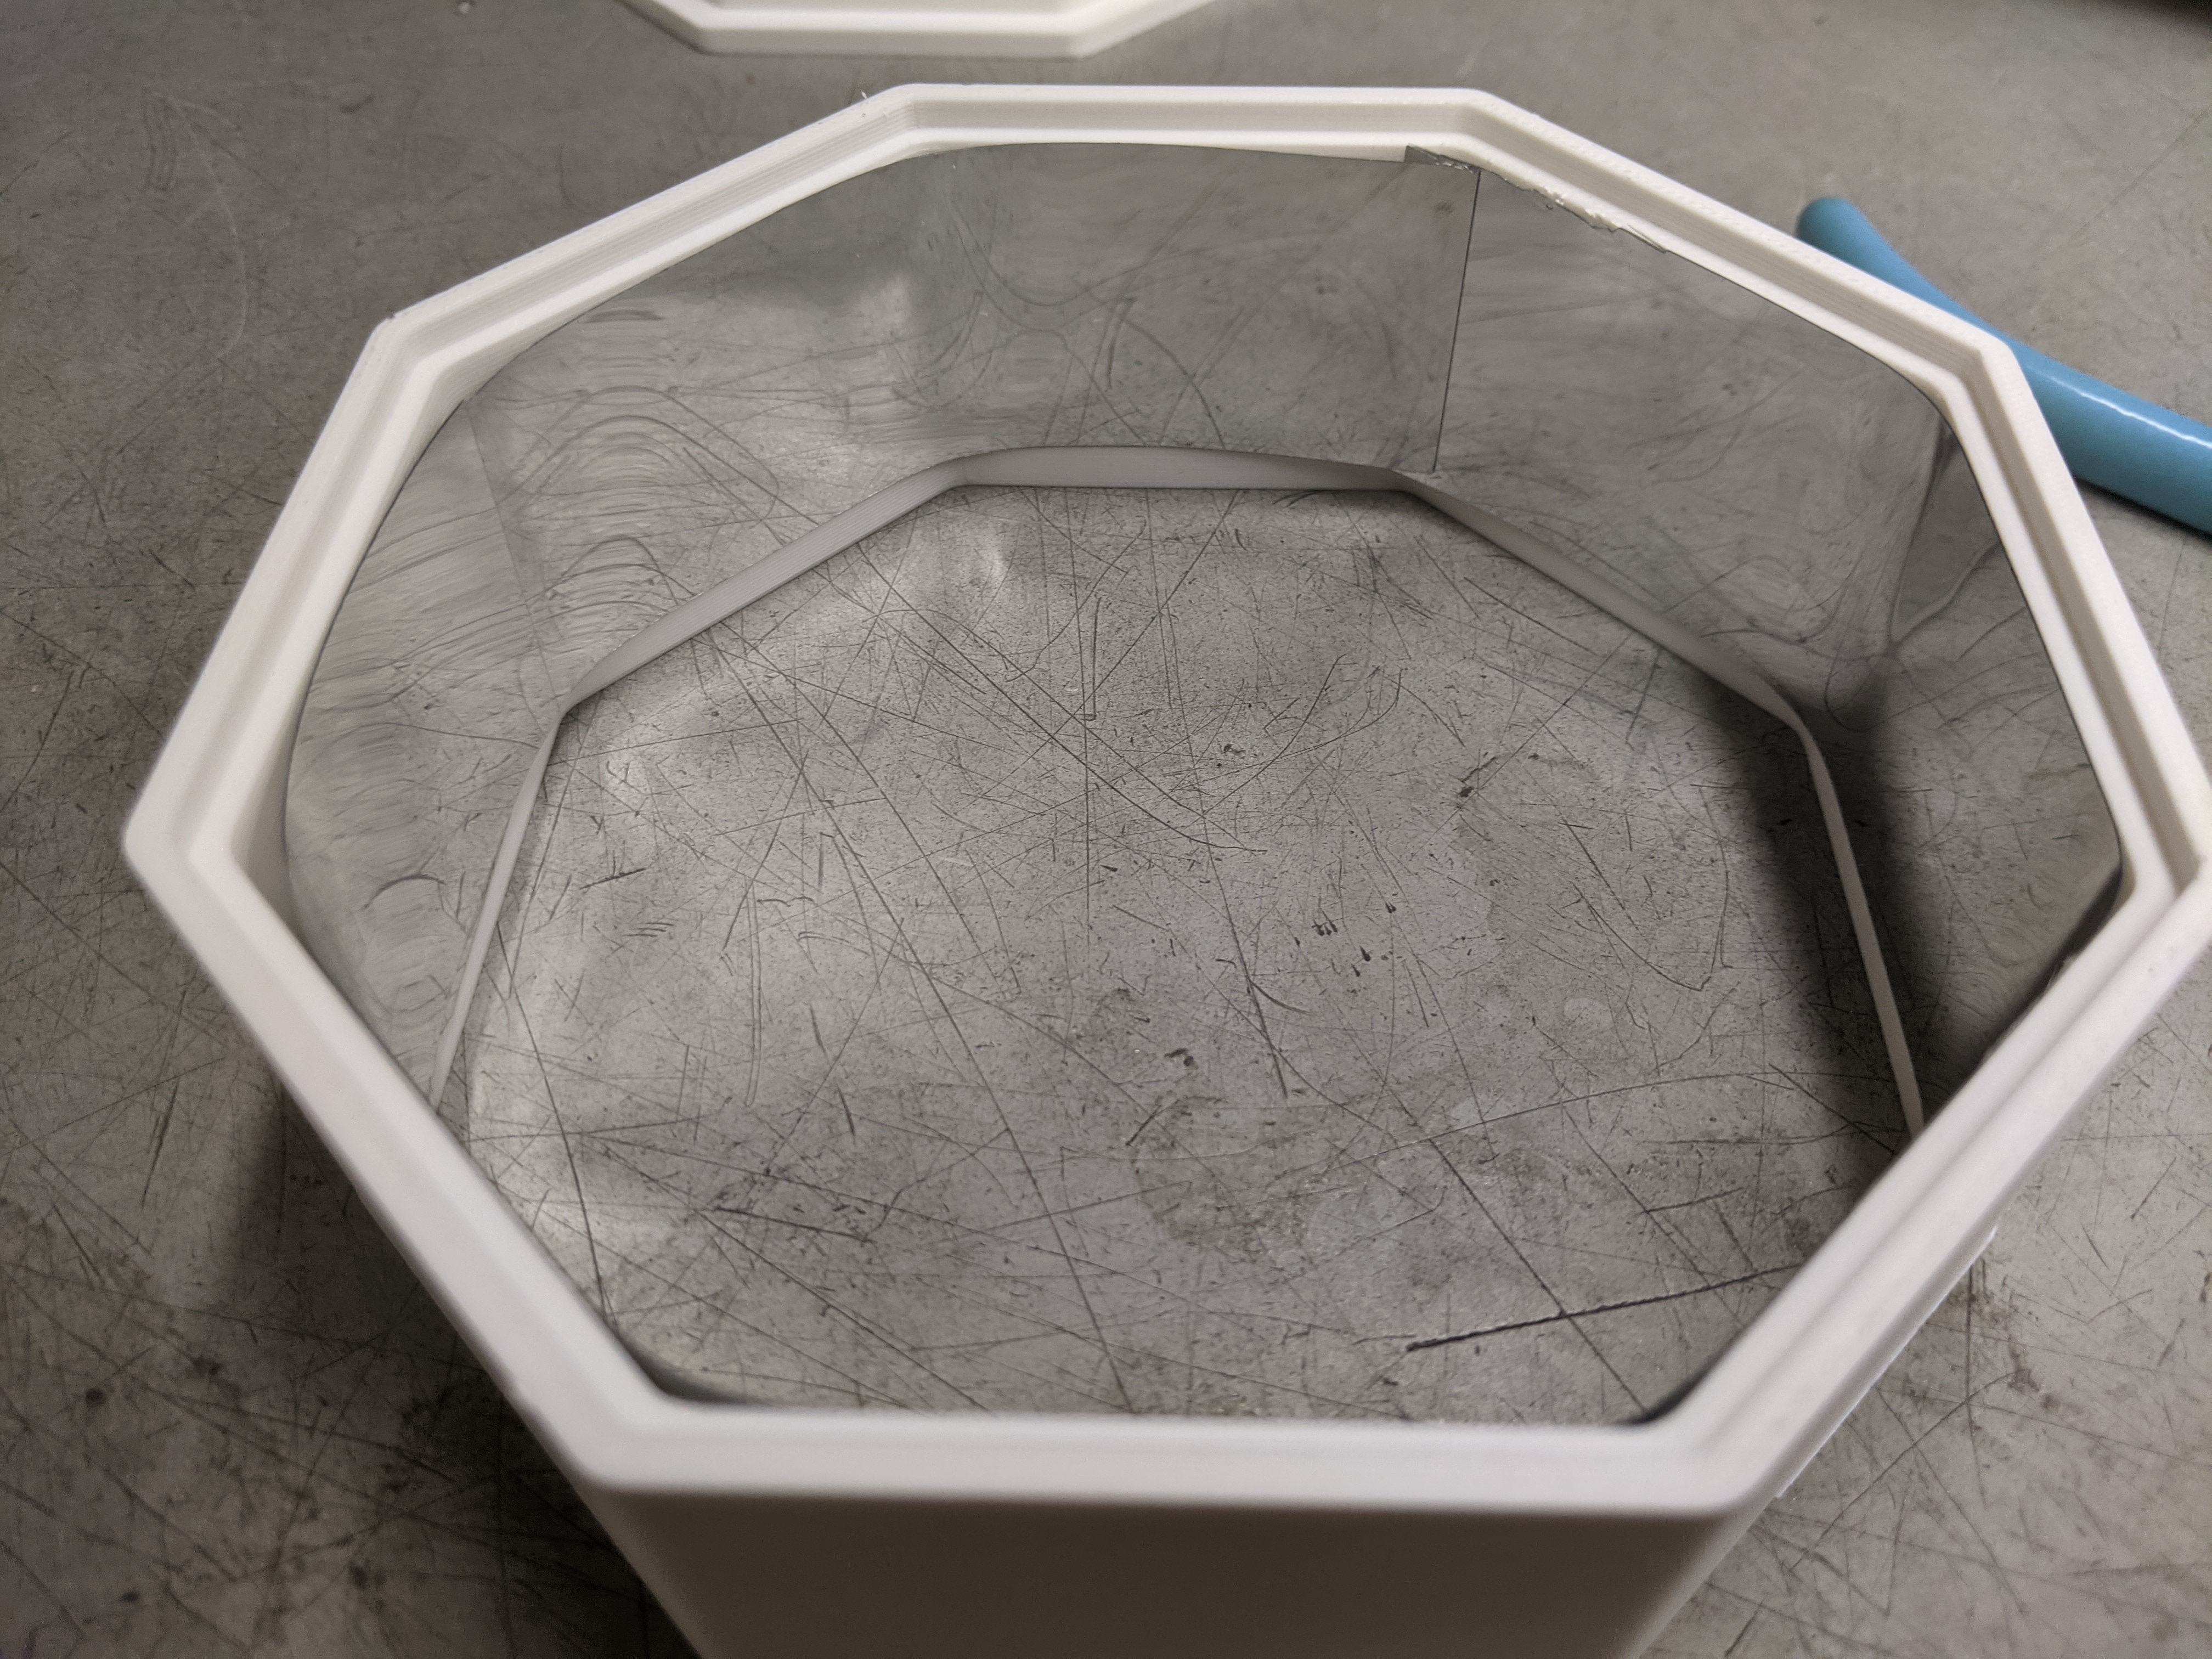
\includegraphics[width=\textwidth]{"./fig9.png"}
	\caption{(A) 4-mL reaction chamber. (B) Chamber lined with reflective material.}
\end{figure}

Once you have both parts printed, cut reflective material to line the inside of the reaction chamber.
Remove the backing and stick the material to the chamber walls (Figure 9A---B).
It is fine to leave overlap around the interior.
The 3D printed vial holder requires no modification.
Your reaction module is now ready for use. 

\clearpage

\subsection{Reactor Driver Electronics} \label{SEC:electronics}

\begin{figure}[H]
	\centering
	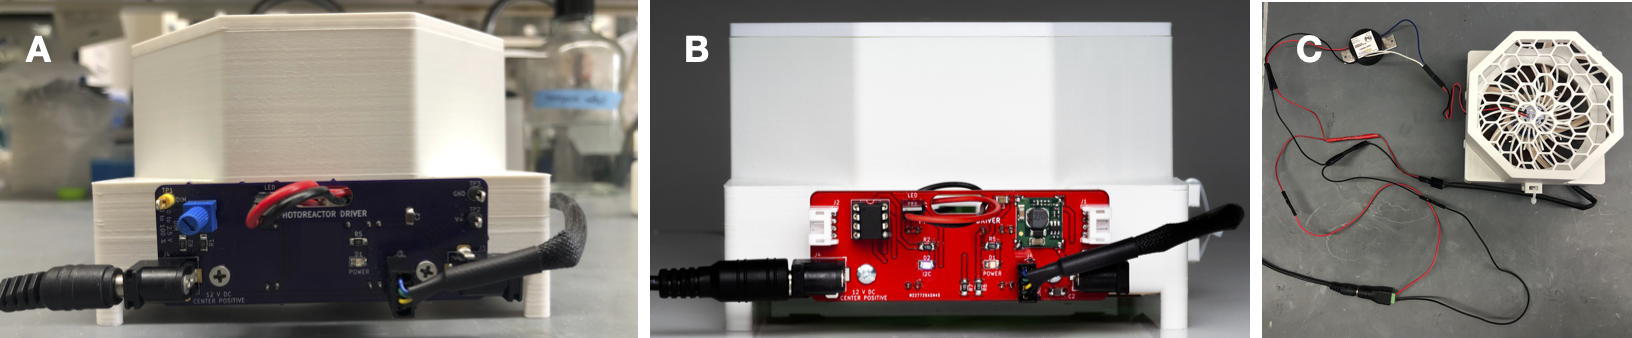
\includegraphics[width=\textwidth]{"./fig10.png"}
	\caption{(A) Analog driver board. (B) Digital driver board. (C) Simple LED driver circuit.}
\end{figure}

A WPP device can be driven using an analog driver circuit board, a digital driver circuit board or a simple electronic circuit with a commercial LED driver (Figure 10).
All provide power to the cooling fan and constant current to the LEDs.
All utilize 1000 mA LED drivers. \textbf{\textit{Each provides different configurational abilities.}}

Both driver boards are built around Mean Well's LDD-1000L LED driver module.
This module delivers constant current up to one amp.
The current delivered can be controlled electronically in several different ways.
Users wishing to understand this design should refer to Mean Well's datasheet.
Refer to the "analog-driver-board" and "digital-driver-board" directories in the online repository for design files for each board.

The analog driver board is designed exceedingly simple to fabricate and use.
The circuit accepts DC 12 V through a barrel jack.
A small knob is used to adjust light intensity.
Fan speed is not adjustable.
\textbf{We recommend chemists interested in adopting the WPP architecture first build and test the analog driver board.} 
Refer to \autoref{SEC:analog-driver} for analog driver board assembly instructions and further explanation.


The digital driver board is made to be incorporated into an I$^2$C-based digital control system.
In addition to power, these boards have 4-pin connectors to carry the I$^2$C serial data.
\textbf{We recommend experienced chemists interested in automation of WPP devices and integration of peripherals to expand device functionality use the digital driver board.} 
Refer to \autoref{SEC:digital-driver} for digital driver board assembly instructions and further explanation.

The simple driver circuit allows for use of any commerical 1000 mA LED driver with the WPP architecture.
Refer to \autoref{SEC:simple-driver} for further explanation.

When interacting with the design files in our online repository you will see several different filetypes.
These circuit boards were designed using KiCad, a free and open source electronics CAD software.
All KiCad files are contained within the ``kicad'' subdirectories.
You may modify and extend these designs however you like.

Those wishing to reproduce our designs should refer to the gerber subdirectory.
Within the gerber directory you will find zip files for each separate version of the printed circuit board (PCB).
You may upload these zip files to PCB manufacturers when ordering copies of our designs.

\clearpage
\subsubsection{Analog Driver Board} \label{SEC:analog-driver}

\begin{figure}[H]
	\centering
	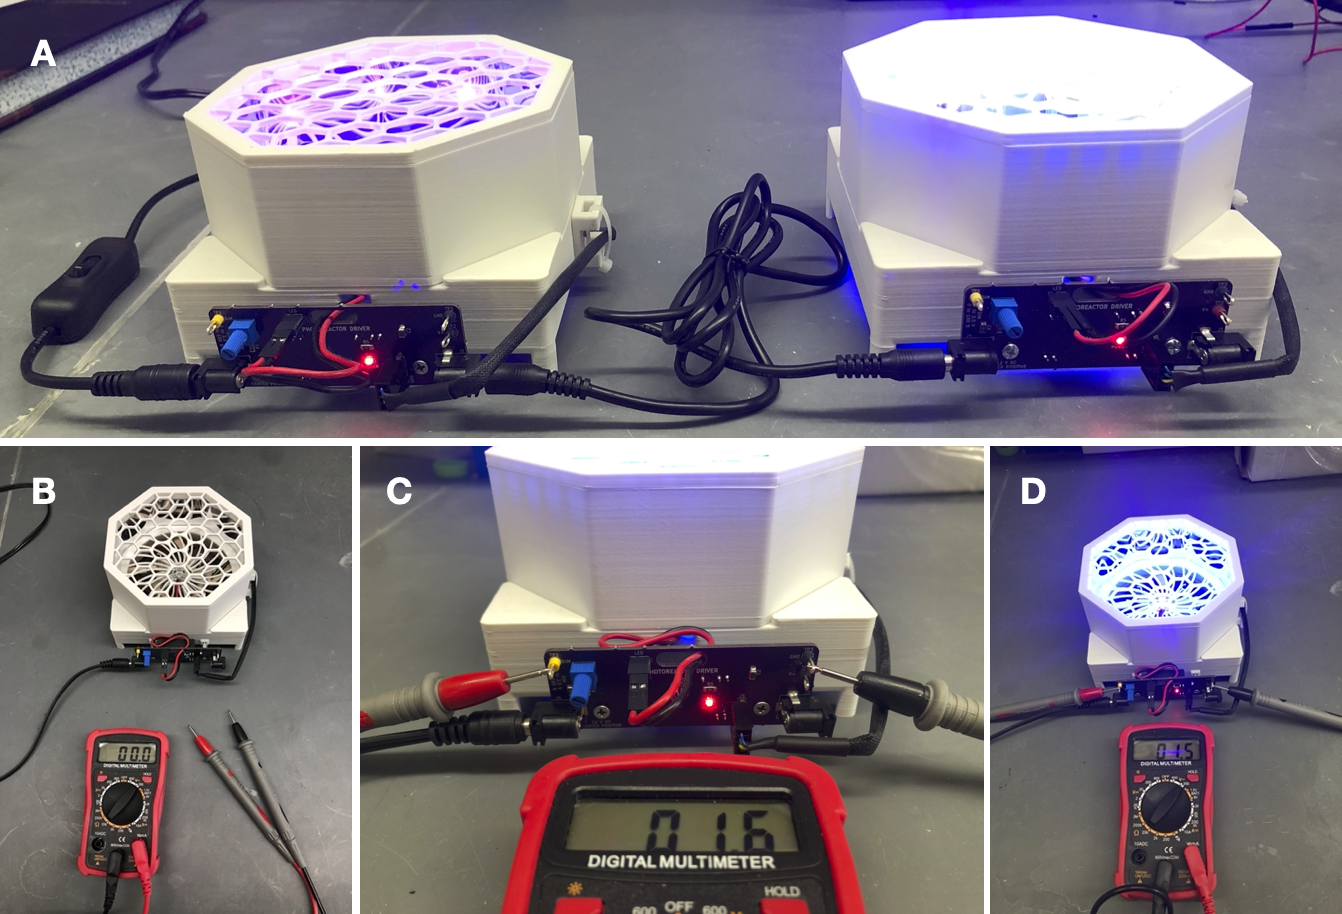
\includegraphics[width=\textwidth]{"./fig11.png"}
	\caption{(A) WPP devices fitted with analog driver boards connected in series. (B) Multimeter and WPP apparatus fitted with analog driver board. (C) Connection of multimeter to test points. (D) WPP apparatus at ~60 percent light intensity (1.5 V test point voltage)}
\end{figure}

\textbf{\textit{Through use of the analog driver board, one can reproducibly control WPP device light intensity.}}
This control is achieved through adjustment of the board-mounted potentiometer.
No software is required, and multiple WPP reactors can be connected in series to a single power source (Figure 11A).
However, fan speed isn’t adjustable and is maintained at maximum.
A full schematic of the analog circuit appears at the end of this section.
A bill of materials appears within the README file of the 'analog-driver-board' subdirectory of the project repository.

Relative light intensity can be determined using the analog driver board test points and a multimeter (Figure 11B-D).
The measured voltage can then be converted to relative light intensity using the values in Table 1.
These values are derived from Mean Well's datasheet for the analog board’s LDD-1000L LED driver.

\begin{table}[H]
	\centering
	\begin{tabular}{ll}
		\centering
		\textbf{Test Point Voltage} & \textbf{Approximate Relative Light Intensity} \\
		2.5                         & 100\%                                         \\
		2.25                        & 90\%                                          \\
		2.00                        & 80\%                                          \\
		1.75                        & 70\%                                          \\
		1.5                         & 60\%                                          \\
		1.25                        & 50\%                                          \\
		1.00                        & 40\%                                          \\
		0.75                        & 30\%                                          \\
		0.5                         & 20\%                                          \\
		0.45                        & 0\%                                          
	\end{tabular}
	\caption{Test point voltage to approximate relative LED intensity conversion. TODO: FIX TABLE FORMATTING.}
	\label{tab:analog-board-conversion}
\end{table}

To fabricate an analog driver board, start by ordering analog board PCBs from a PCB manufacturer. Your PCB manufacturer will send you bare boards of the type seen in Figure 12A. 

\begin{figure}[H]
	\centering
	\includegraphics[width=\textwidth]{"./fig12.png"}
	\caption{(A) Blank analog driver board. (B) Analog driver board with labeled surface mount components.}
\end{figure}

Begin by adding the surface mount components. 
Refer to the analog driver schematic for part identities.
We recommend using thin solder, e.g. 0.015''.
The surface mount resistors and capacitors have no polarity.
However, the power indicator LED does have a polarity---ensure that the small green line points towards ground (left).
Once done your analog board should look that depicted in Figure 12B. 

\begin{figure}[H]
	\centering
	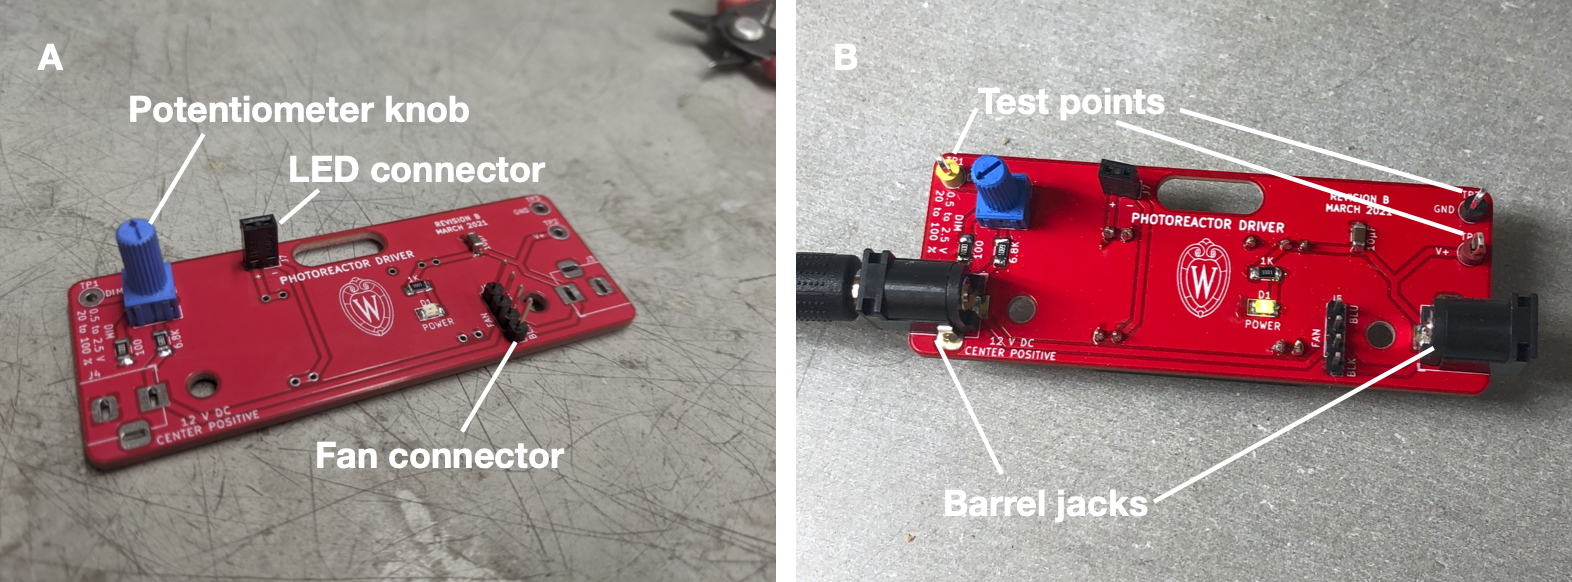
\includegraphics[width=\textwidth]{"./fig13.png"}
	\caption{(A) Analog driver board with potentiometer and connectors (B) Powered analog driver board.}
\end{figure}

Next, solder on the connectors and the potentiometer knob (Figure 13A).
From now on we recommend standard gage solder, e.g. 0.031''.
You can then add the barrel jacks and test points. 
With these added you may plug in your board into power for the first time.
Either barrel jack can be plugged in.
You should see your power indicator LED illuminate (Figure 13B)

\begin{figure}[H]
	\centering
	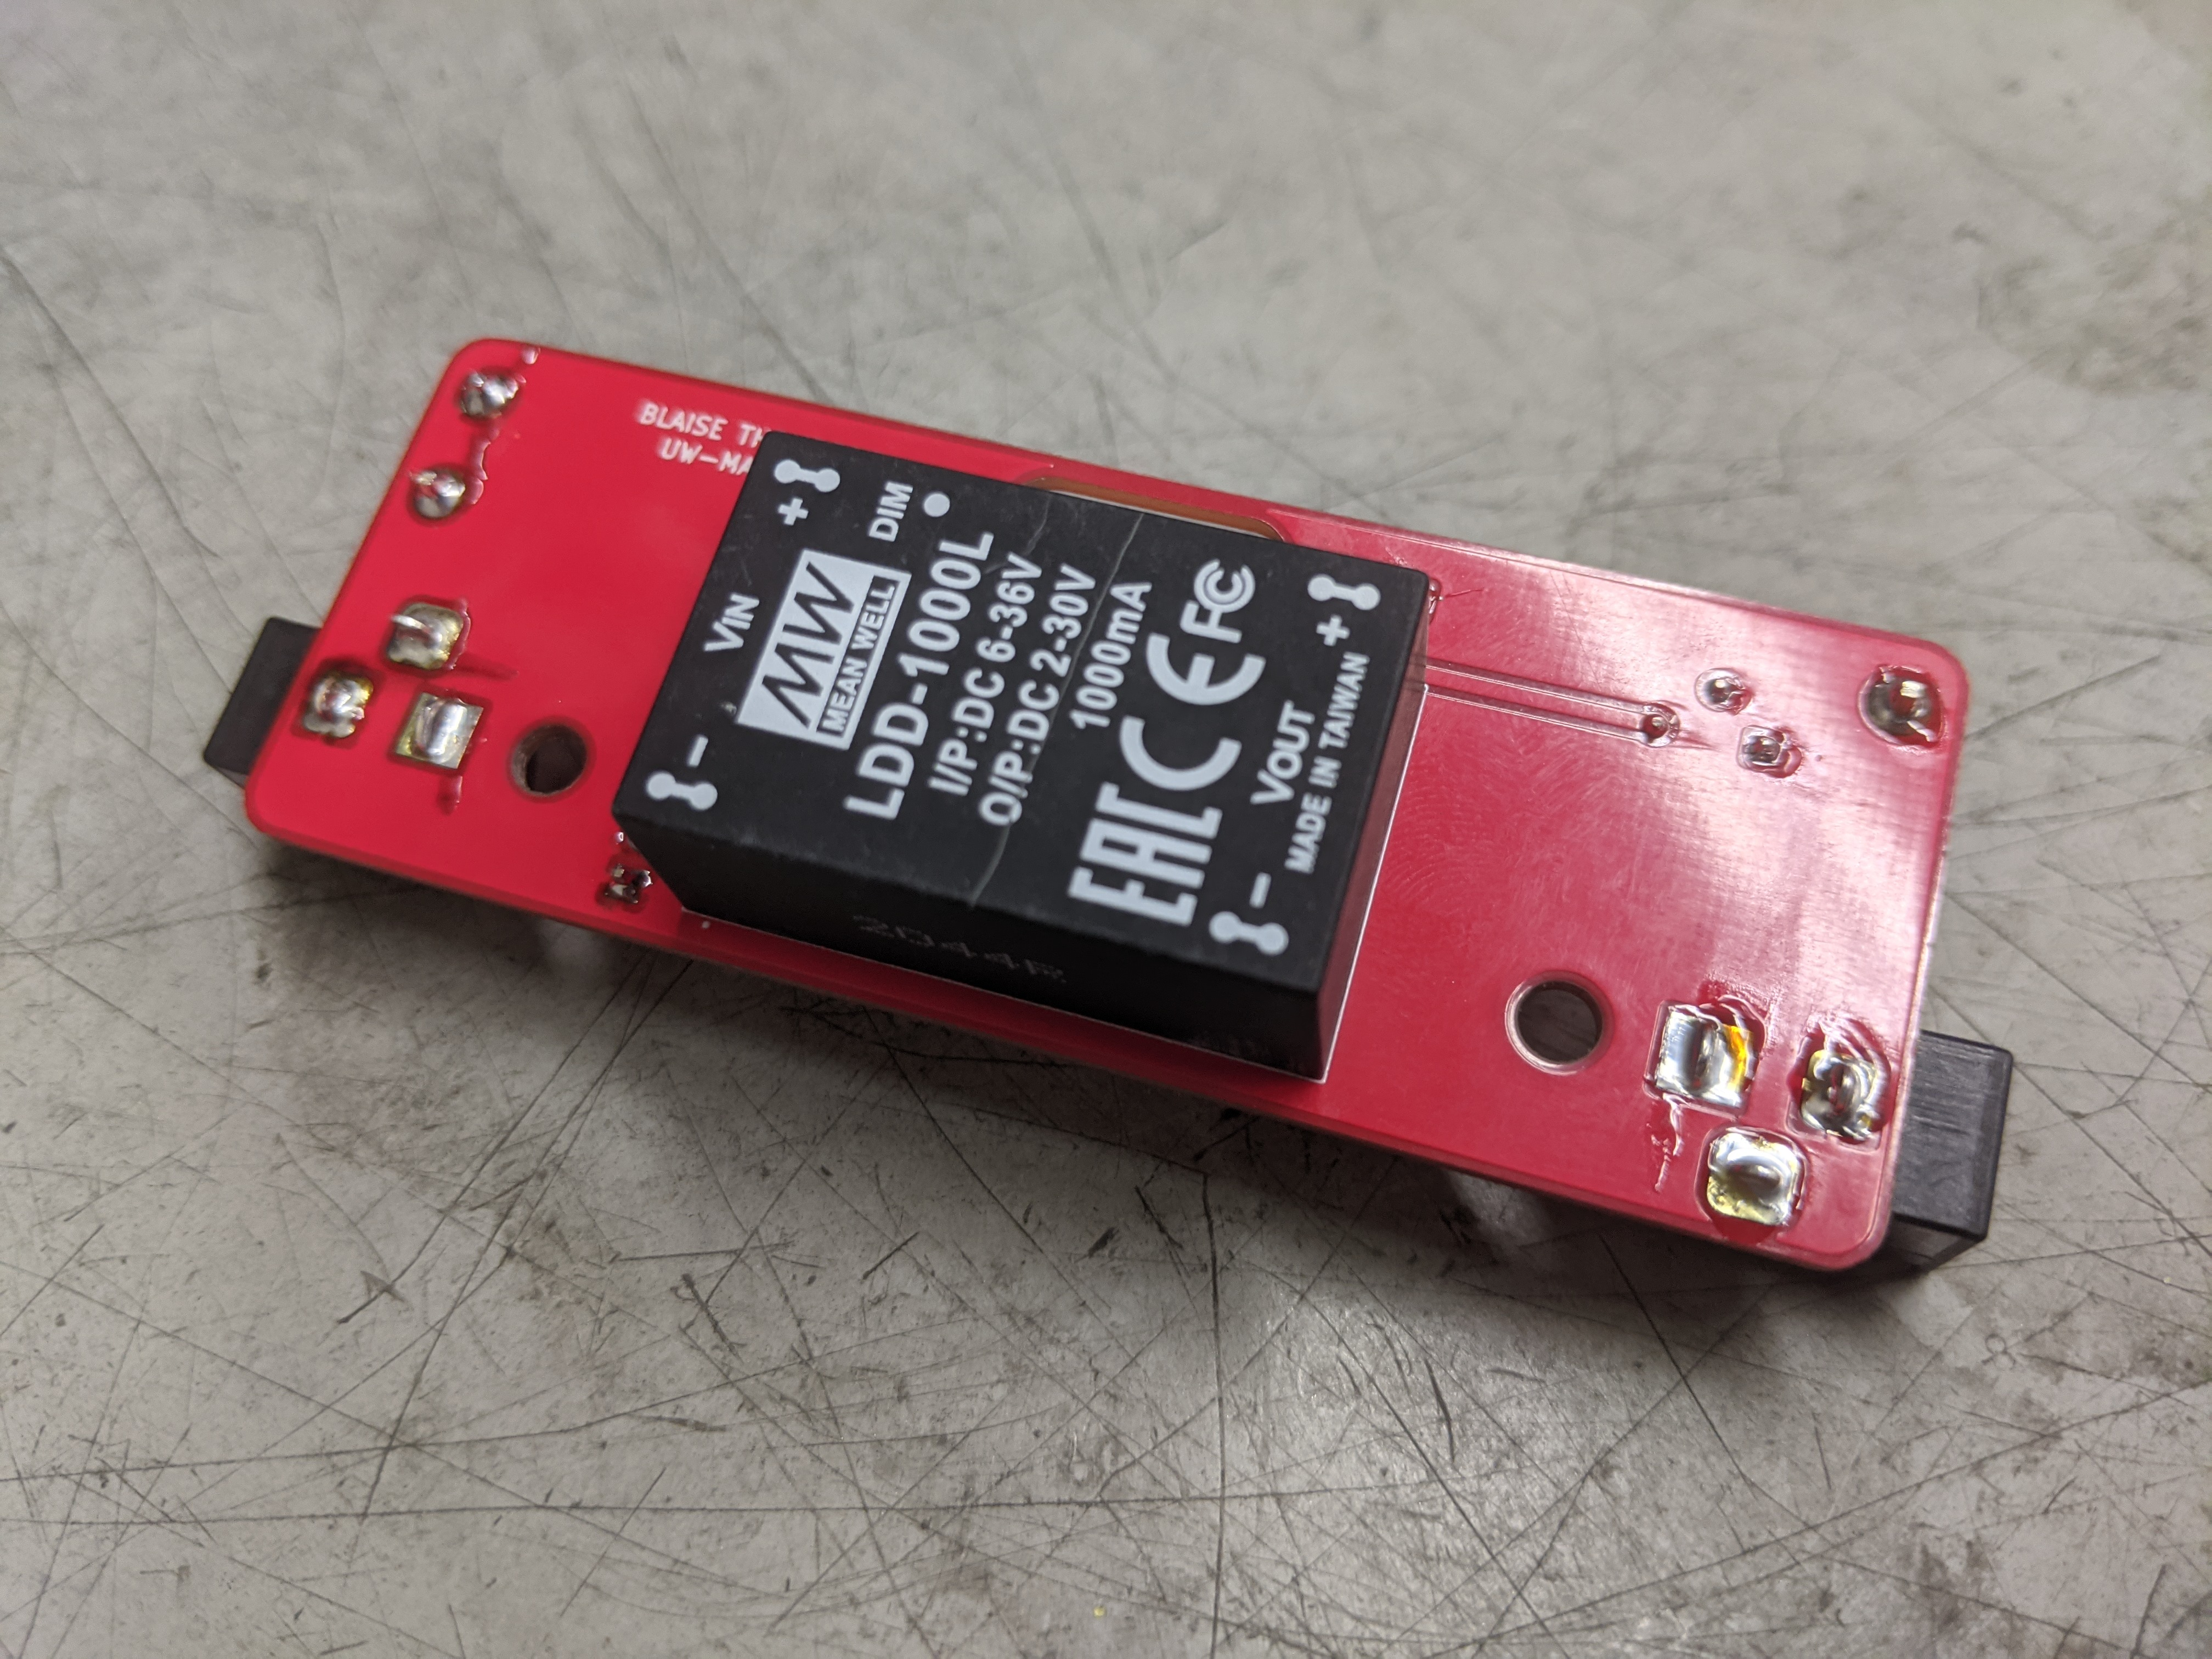
\includegraphics[width=0.5\textwidth]{"./fig14.jpg"}
	\caption{(A) Blank analog driver board. (B) Analog driver board with labeled surface mount components.}
\end{figure}

Finally, solder on the Mean Well LDD-100L LED driver (Figure 14).
This component goes on the back of the analog driver board. 
The analog driver board is now ready for use.

\includepdf[landscape=true]{"../analog-driver-board/driver.pdf"}

\subsubsection{Digital Driver Board} \label{SEC:digital-driver}

\begin{figure}[H]
	\centering
	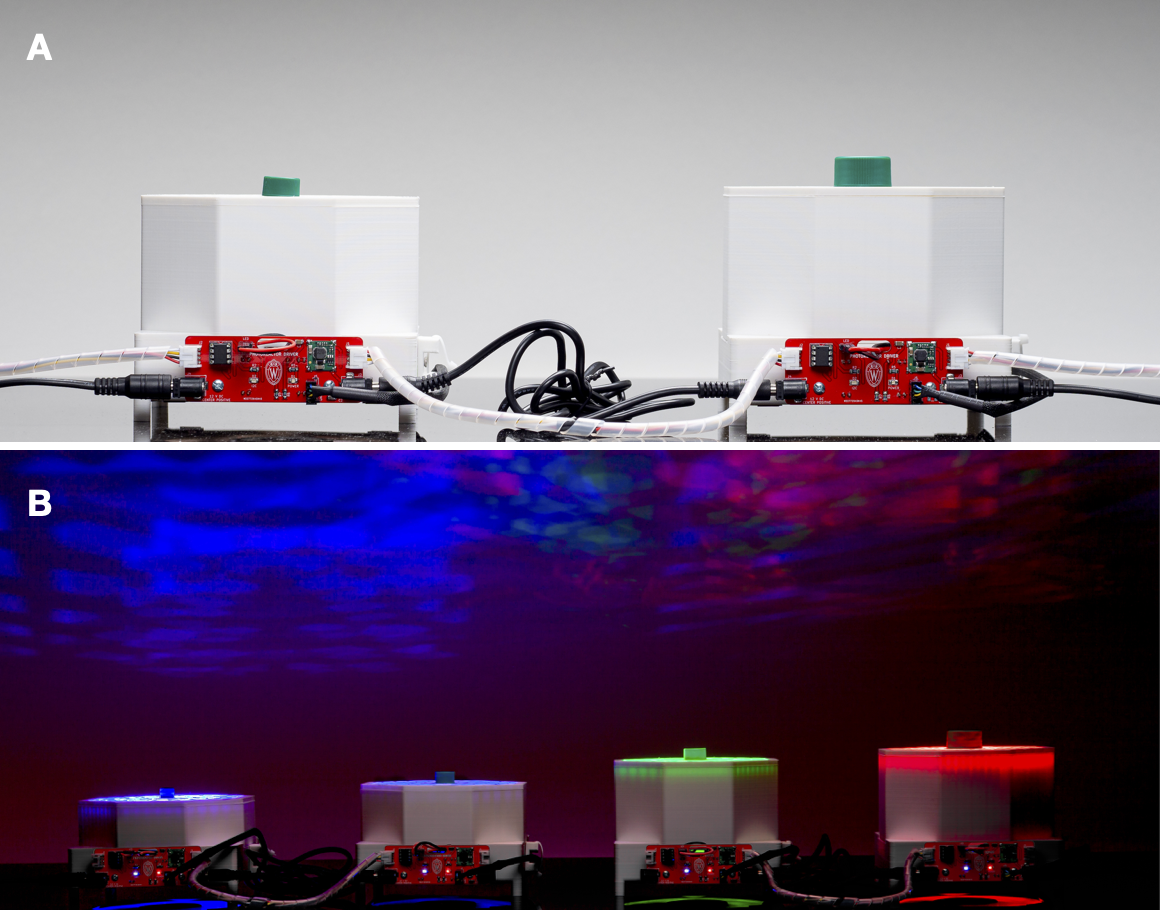
\includegraphics[width=\textwidth]{"./fig15.png"}
	\caption{(A) WPP devices fitted with digital driver boards connected in series. (B) Powered WPP devices connected in series.}
\end{figure}

The digital driver circuit can be controlled from a computer or some other digital device.
We built our driver to work over I2C, consistent with an emerging standard for many ``maker'' products.
While the physical connectors may be different, our digital circuit is compatible with the following systems.

\begin{itemize}
  \item \href{https://learn.adafruit.com/introducing-adafruit-stemma-qt}{Adafruit STEMMA}
  \item \href{https://www.sparkfun.com/qwiic}{Sparkfun Qwiic}
  \item \href{https://www.seeedstudio.com/category/Grove-c-1003.html}{Seeed Grove}
\end{itemize}

Through use of the digital driver board, one can control WPP device light intensity and fan speed.
This control is achieved by connecting a control unit, like an Arduino Uno, to the digital driver board using custom software.
Multiple WPP devices with digital driver boards can be connected to a single control unit and power supply (Figure 5).
Open-source software for interfacing digital driver boards and Arduino Uno control units is provided in the project repository.
Instructions for implementing this software and controlling WPP devices using it are in the fabrication guide.
Other I2C peripherals can be connected to digital driver boards to expand functionality, but software must be produced to interface with them.

\begin{center}
  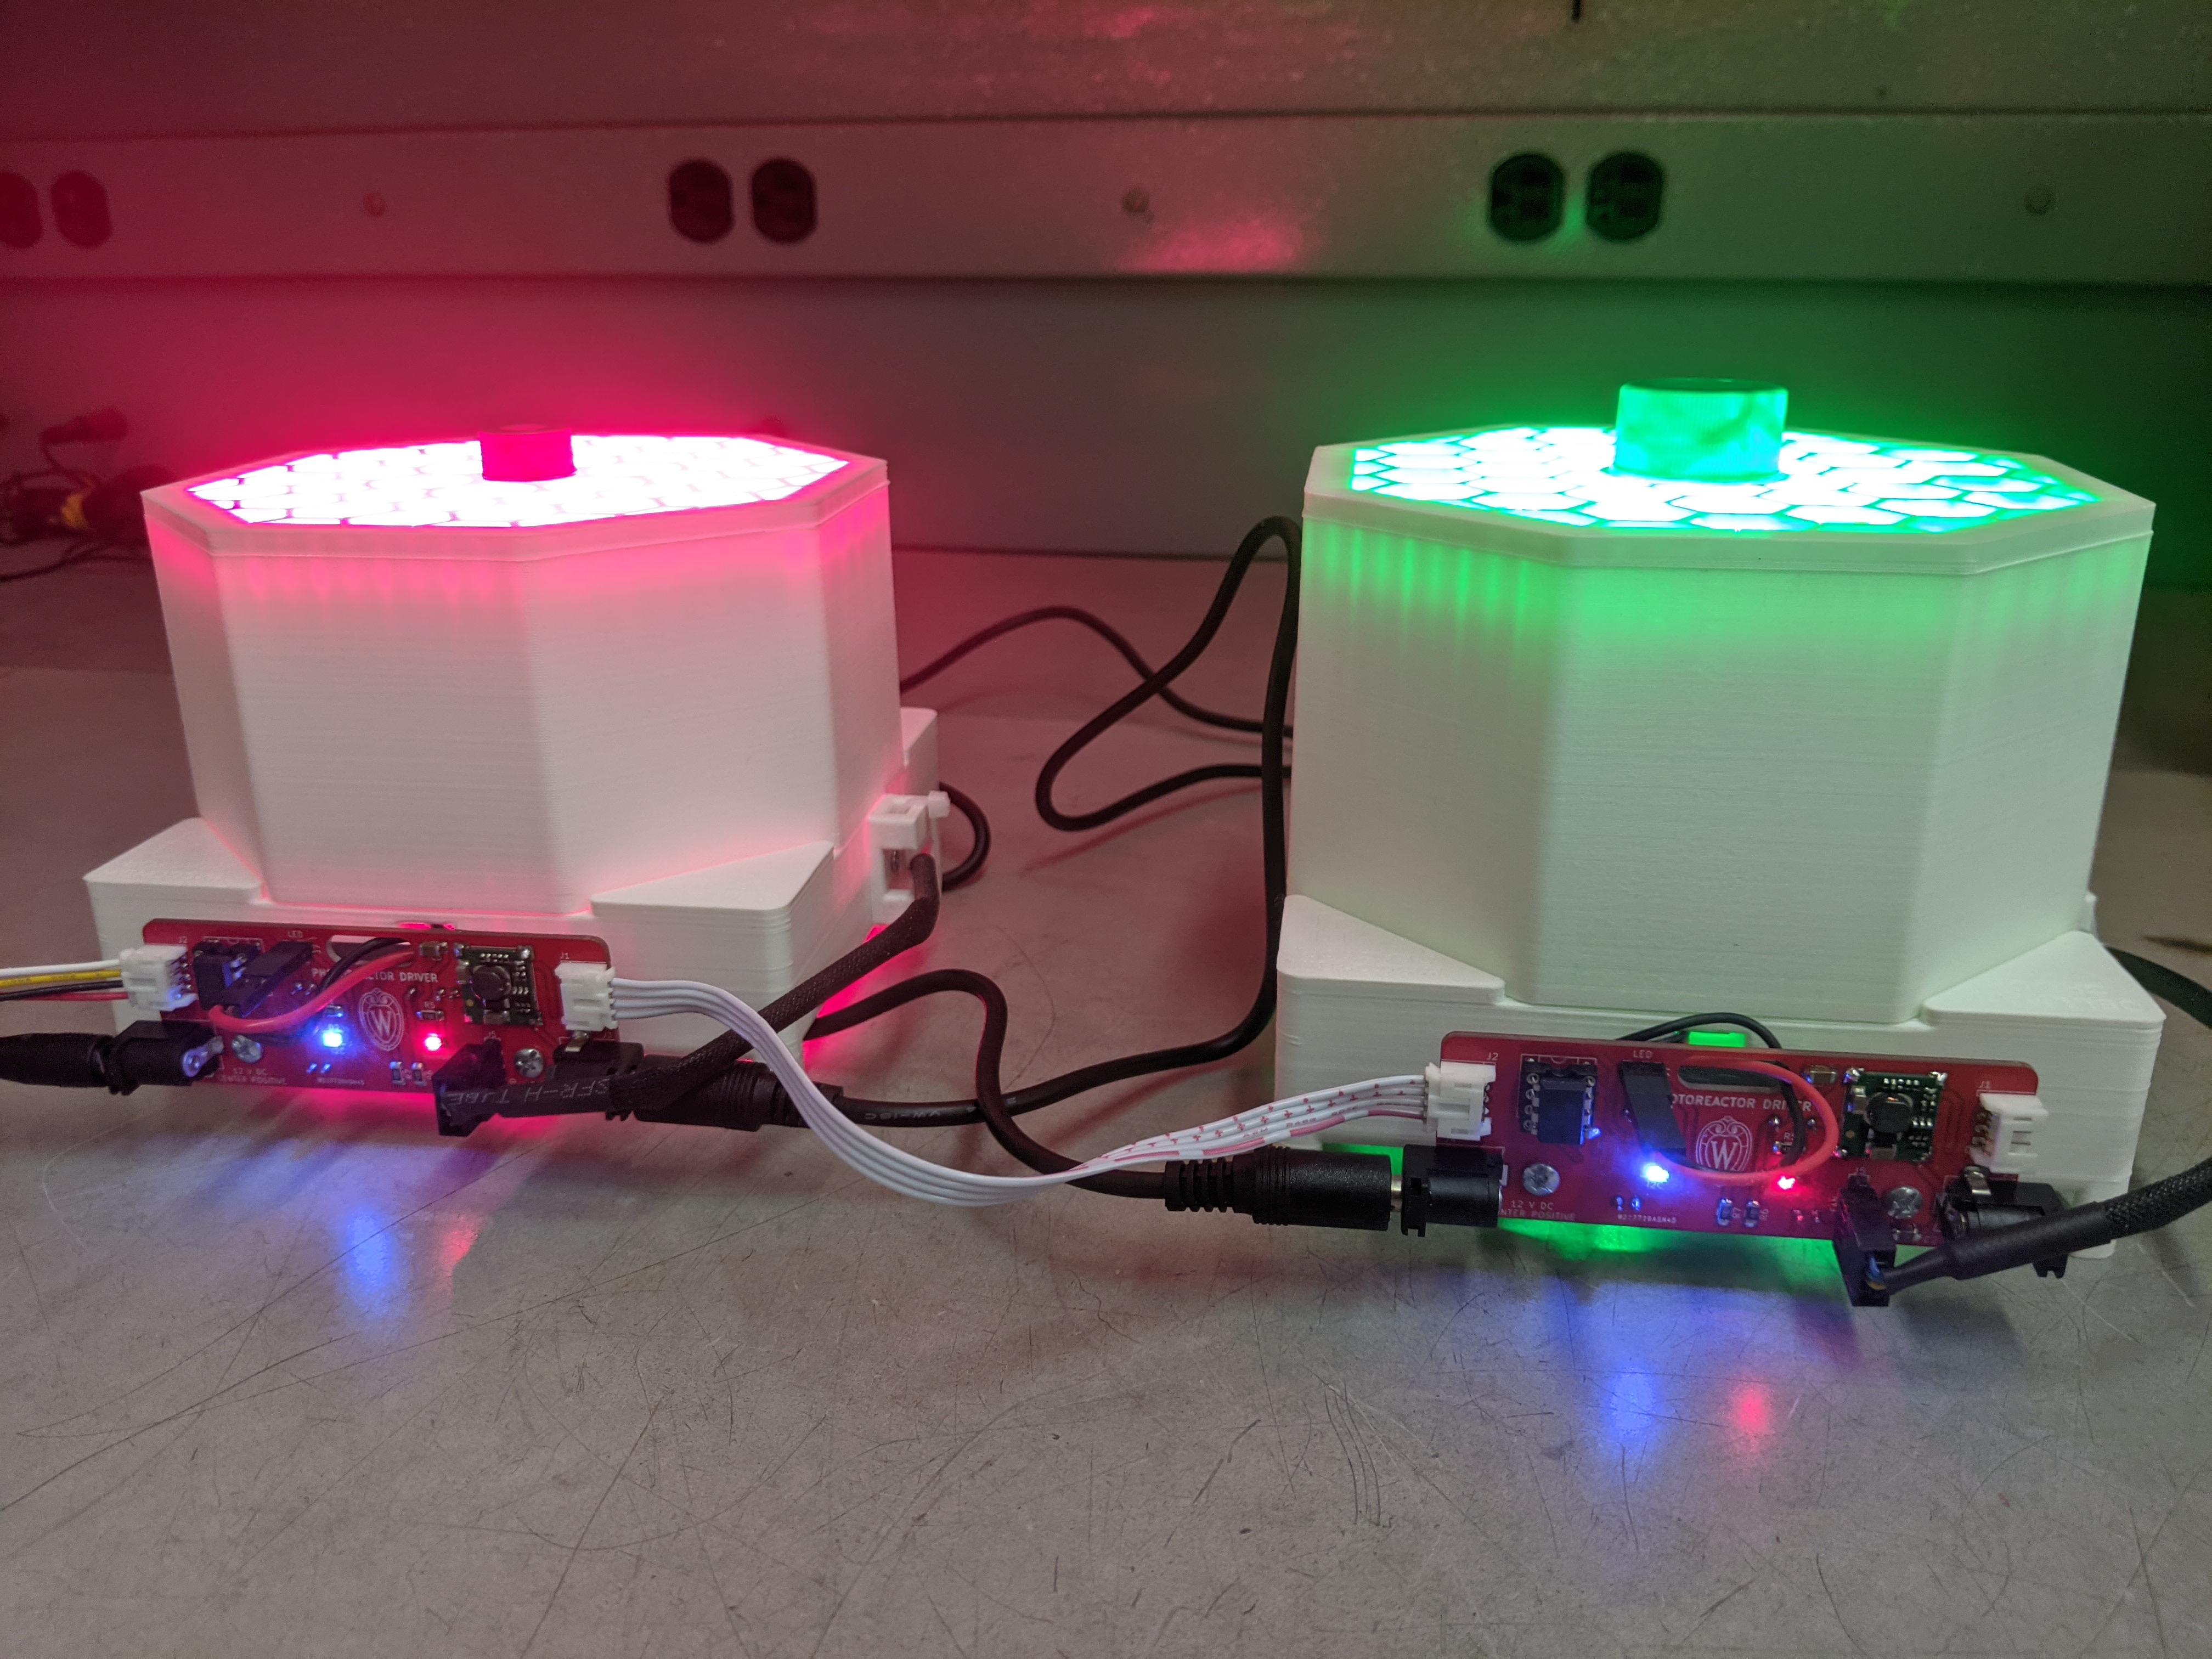
\includegraphics[width=\textwidth/2]{"./digital-wired.jpg"}
\end{center}

Each digital driver is based around an ATtiny85 microcontroller acting as an I2C peripheral.
Multiple digital driver boards may be ``networked'' together onto one I2C bus by simply daisy-chaining the boards together, as shown above.
In such a use-case you must choose a unique I2C address for each ATtiny85 peripheral.

\begin{center}
  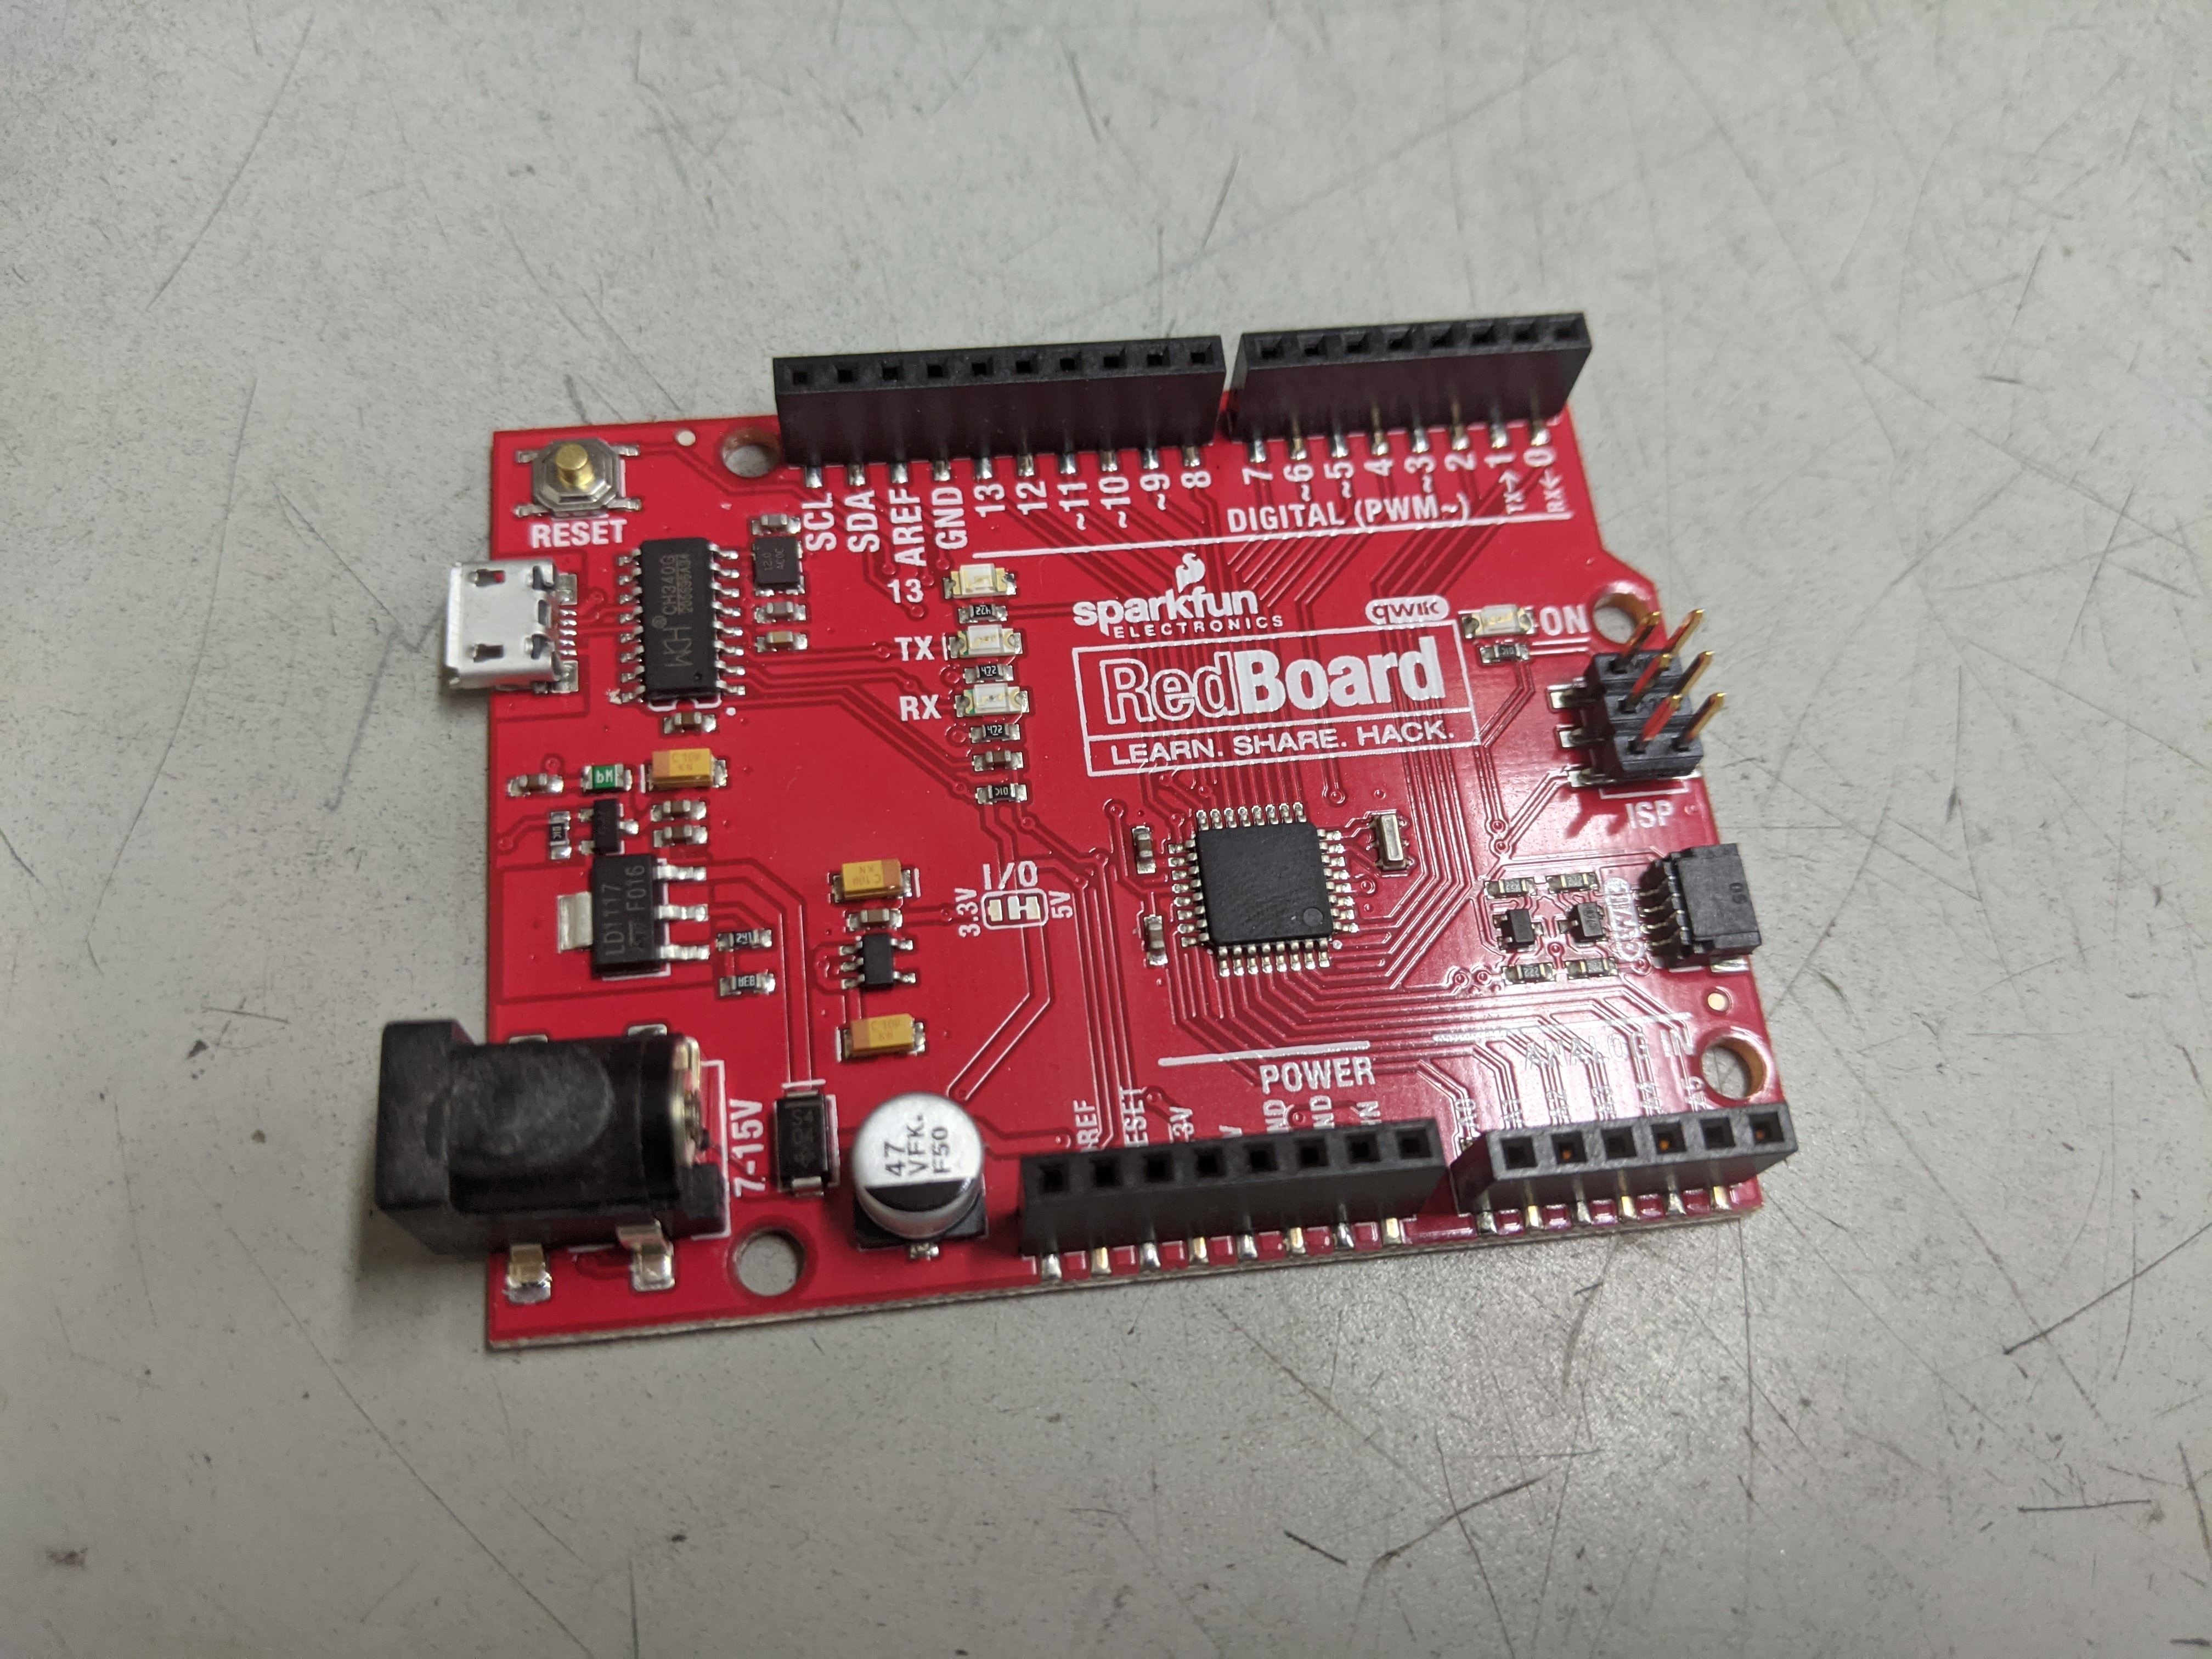
\includegraphics[width=\textwidth/2]{"./redboard.jpg"}
\end{center}

There are many ways to interface with the I2C bus.
We have used a SparkFun RedBoard, pictured above.
You may find an example within the online repository that dynamically controls both the LED intensity and fan speed.

\includepdf[landscape=true]{"../digital-driver-board/driver.pdf"}

\subsubsection{Simple Driver Circuit} \label{SEC:simple-driver}

\begin{figure}[H]
	\centering
	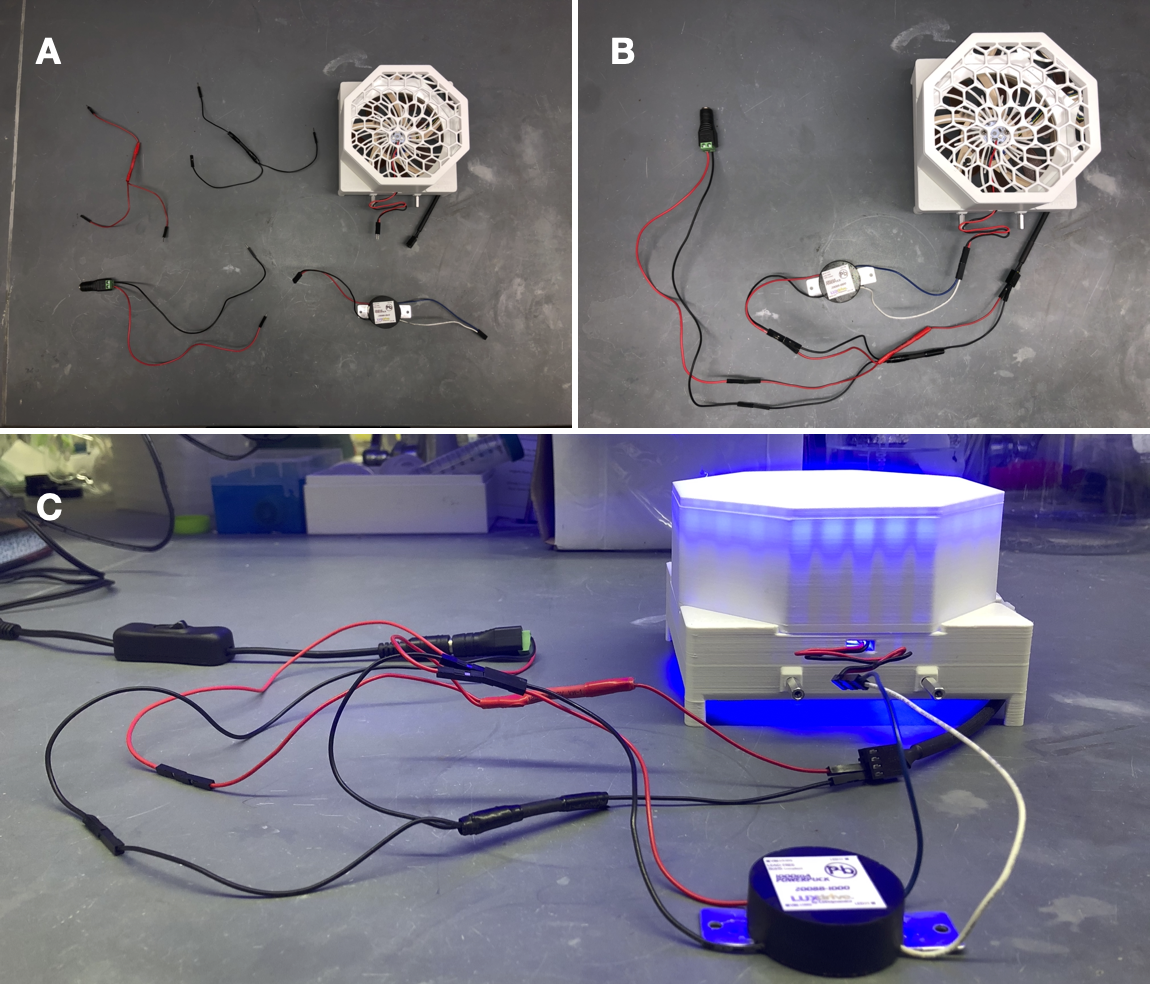
\includegraphics[width=\textwidth]{"./fign7.png"}
	\caption{(A) Unassembled pieces of the simple LED driver circuit integrating a LUXdrive 1000mA PowerPuck LED driver (Part number: 2008B-1000). (B) Assembled circuit. (C) Powered circuit.}
\end{figure}

The LED driver circuit shown in Figure N is the simplest way to drive a WPP apparatus.
Neither light intensity nor fan speed can be configured when using the simple LED driver circuit.
Both are maintained at maximum power.
However, no circuit board fabrication is required, and any commercial 1000 mA LED driver can be used.

\section{Operation}

Once a WPP apparatus is configured with the desired photon source, reaction module and reactor driver, it is ready to drive photoreactions.

\begin{figure}[H]
	\centering
	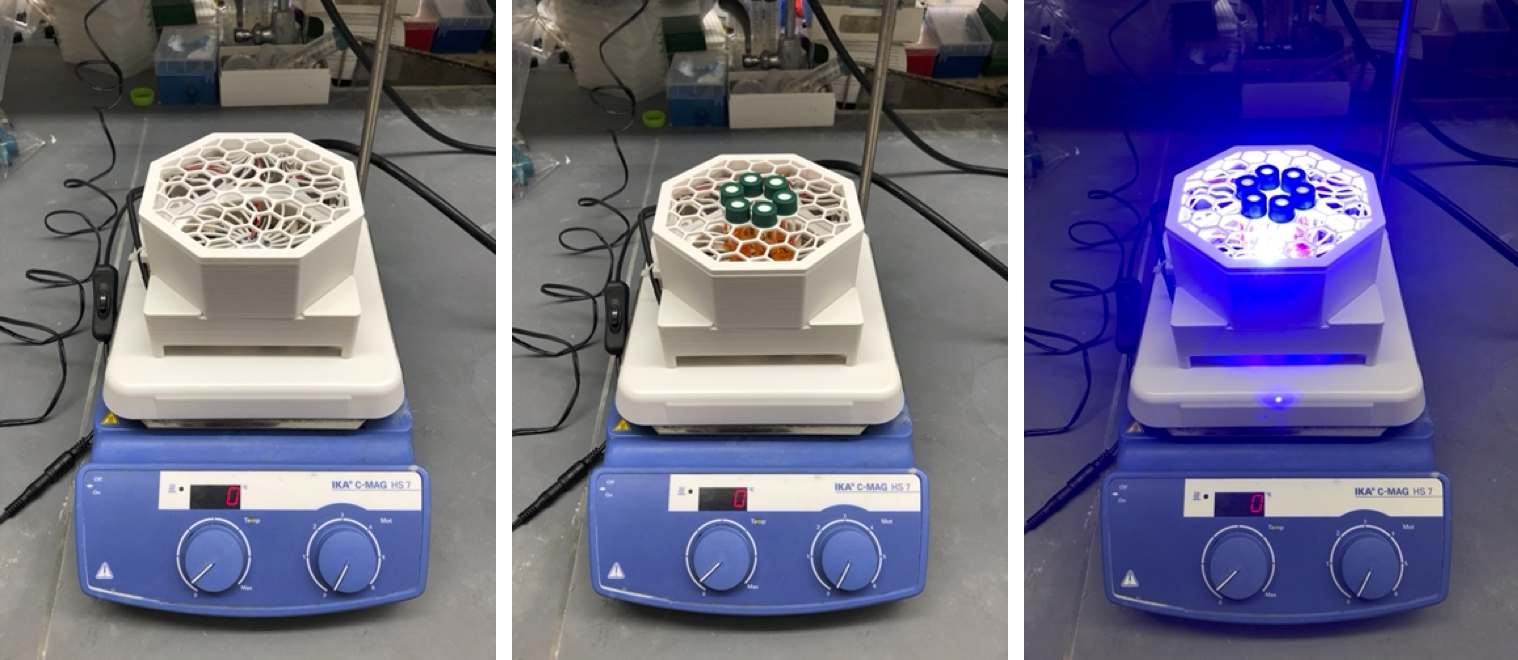
\includegraphics[width=\textwidth]{"./fign8.png"}
	\caption{A WPP apparatus with a 450 nm photon source, 4 mL reactor module and digital driver board on a standard laboratory stir plate conducting 6 simultaneous photoreactions in the multiple reaction configuration.}
\end{figure}


To conduct a photoreaction using a WPP device, an assembled apparatus should be placed on a lab stir plate, to provide reaction mixture stirring, and reaction vessels should be inserted into the apparatus in the desired layout (Figure 8).
The 130 by 130 mm footprint of the WPP architecture is compatible with typical stir plates.
A standard 12 V power supply can then be plugged into the reactor driver to turn on the device and start reaction.
A single 12V 2 A power supply is sufficient to drive 2 WPP devices simultaneously.
A switch can be installed between the WPP apparatus and power supply to provide power switching.

Reaction and photon source cooling is provided by the fan integrated into the base.
Additional cooling can be achieved through placement of fans above the WPP apparatus or by placing a WPP device on a stir plate within a refrigerator or cold room.

Once finished, the WPP apparatus can be switched off by simply unplugging it and disassembled for storage.

\section{Documentation}

Users should report the following for each photon source used:

    (1) Max emission wavelength for LEDs.
    (2) Manufacturer and part number for LEDs.
    (3) Supplier and part number for LED star (if commercial).

This information enables precise reproduction of WPP photon sources. Characterization of a photon source’s emission profile using a spectrometer is recommended but not required for reproduction. Emission profiles for commercial LEDs are supplied in part datasheets provided by manufacturers. A list of WPP-compatible LED stars exhibiting emission profiles across the visible range is provided in the project repository.

Users should provide and report the following for each module used:

    (1) Original CAD designs for both module parts.
    (2) 3D-printable models for both module parts.
    (3) Photos of each reaction vessel placement configuration.
    (4) Manufacturer and part number for reaction vessel.

These provisions enable precise reproduction of reaction modules. Documenting the height a vessel is held above the photon source is recommended but not required for reaction module reproduction. All reaction modules provided in the project repository hold vessels a standardized 7 mm above the photon source.

Users should report the following when an analog driver board is used:

    (1) Measured test point voltage.
    (2) Relative intensity at which LEDs are driven (0 to 100%).

These provisions enable precise reproduction of reaction conditions for transformations carried out using WPP devices fitted with analog driver boards.

Users should provide and document the following when a digital driver board is used:

    (1) Software used to operate the digital driver board, control unit and any other peripherals.
    (2) Relative intensity at which LEDs are driven (0 to 100%).
    (3) Relative fan speed (0 to 100%).

These provisions enable precise reproduction of reaction conditions for transformations carried out using WPP devices fitted with digital driver boards

Users should report the following when a simple LED driver circuit is used:

    (1) Manufacturer and part number for LED driver.

This information enables reproduction WPP devices fitted with the simple LED driver circuit.

\section{Safety}

WPP reactors utilize high-intensity light emitting diodes (LED) that can cause eye damage if proper safety precautions are not observed.
Light-filtering safety glasses should be worn whenever a WPP apparatus photon source is powered.
Care must be taken to use safety glasses protective against the specific emission wavelengths of the photon source.

\end{document}
